\chapter{Implementation and Evaluation}
\label{sec:implementation}

In this chapter, I will present a prototype system that realizes \sysname{}
design and three non-trivial wide-area streaming applications with evaluations.

\section{Framework}
\label{sec:framework}

The proposed \texttt{maybe} APIs are not language specific. Although the
prototype is built on top of Rust, it can be easily implemented in other
existing frameworks. I chose Rust mainly because of the memory safety guarantee
and the efficient runtime. First, Rust's memory safety guarantee ensures
applications to run continuously for an extended period of time. This eliminates
a large body of bugs caused by memory corruption; these bugs often require
careful programming analysis for traditional system programming languages such
as C or C++. Besides, the zero-cost abstraction offers runtime efficiency. It
removes the possibilities of tail latency that will happen in garbage-collection
(GC) languages, especially when uncoordinated GC kicks
in~\cite{maas2016taurus}. There are some additional features about Rust that
made the prototype appealing, such as the type enforcement on the function
argument passed to the \texttt{maybe} APIs.

All operators implement the \texttt{Stream} trait that has an associate type
\texttt{Item} and a core function \texttt{next}. The \texttt{next} function,
when invoked, will return a \texttt{Datum} that is a union type of
\texttt{Stream::Item} or \texttt{Error}. Imagine a source operator that
implements the \texttt{Stream} trait, applications can keep calling
\texttt{next} function and will receive the data under normal conditions. When
an error occur, the \texttt{next} function will return an \texttt{Error} that
contains the cause of the error.

The \texttt{maybe} function is one operator that transforms a stream (the first
argument \texttt{self}) into an object of \texttt{Maybe} type. The \texttt{self}
argument means that this function can be invoked on an object of this
type. Imagine a data structure that implements the \texttt{Stream} trait and we
have an instantiated object called \texttt{foo}, then you can use
\texttt{foo.maybe(...)} where \texttt{foo} will be the \texttt{self}.

Two other arguments taken by \texttt{maybe} are almost a direct translation of
the API specification in the design (\autoref{tab:operators}). While the design
uses a vector for knobs, the Rust implementation is more general: any type
(including vector) that implements \texttt{IntoKnob} trait can be used as the
knob. The function argument here is \texttt{FnMut}, which is one type of the
call operators (often a closure) that is allowed to have side effects---it takes
mutable references to the closed environment. Interested readers should refer to
Rust documentations for Rust closures.

\begin{lstlisting}
    pub trait Stream {
        type Item;
        fn next(&mut self) -> Datum<Self::Item, Error>;

        fn maybe<K, F>(self, opts: K, f: F) -> Maybe<Self, F>
            where Self: Sized,
                    K: IntoKnob,
                    F: FnMut(K::Item, Self::Item) -> Self::Item {

             // omitted
        }
    }

    pub trait IntoKnob {
        fn into_knob(self) -> Knob;
    }
\end{lstlisting}

Developers can then use the above API with arbitrary user-defined functions.

\begin{lstlisting}
    let quantized_stream = vec![1, 2, 3, 4]
        .into_stream()
        .maybe(vec![2, 3], |knob, d| d / knob);
        .collect();
\end{lstlisting}

The snippet above shows how a quantization degradation can be
implemented. First, a vector of values is converted into a stream object. Then a
\texttt{maybe} operator is chained after the stream; it's configured with a knob
value (2 or 3) and a function (closure in this example) that does an integer
division (quantization). The function \texttt{collect} will run this stream and
output the result as a vector. In this example, depending on the degradation
level, the output stream could either be [1, 2, 3, 4] (no degradation), [0, 1,
1, 2] (quantized by 2), or [0, 0, 1, 1] (quantized by 3).

In the implementation, we've also extended the basic API set for common
operations. For building video processing applications, we've built a
specialized \texttt{maybe\_downsample} operator can that wraps
\texttt{downsample} function:

\vspace{0.5em}
\texttt{fn downsample(res: (usize, usize), image: Mat) -> Mat;}
\vspace{0.5em}

In our current prototype, an application built with \sysname{} runs as a single
process and the entire processing pipeline---without explicit separation of
client and server---is often specified in a single main file. The execution mode
(profiling, runtime as client or runtime as server) is configured with command
line arguments or environment variables. Our deployment manager is currently a
shell script using Docker container.

\section{Building \sysname{} Applications}
\label{sec:build-appl}

\begin{figure*}
  \centering
  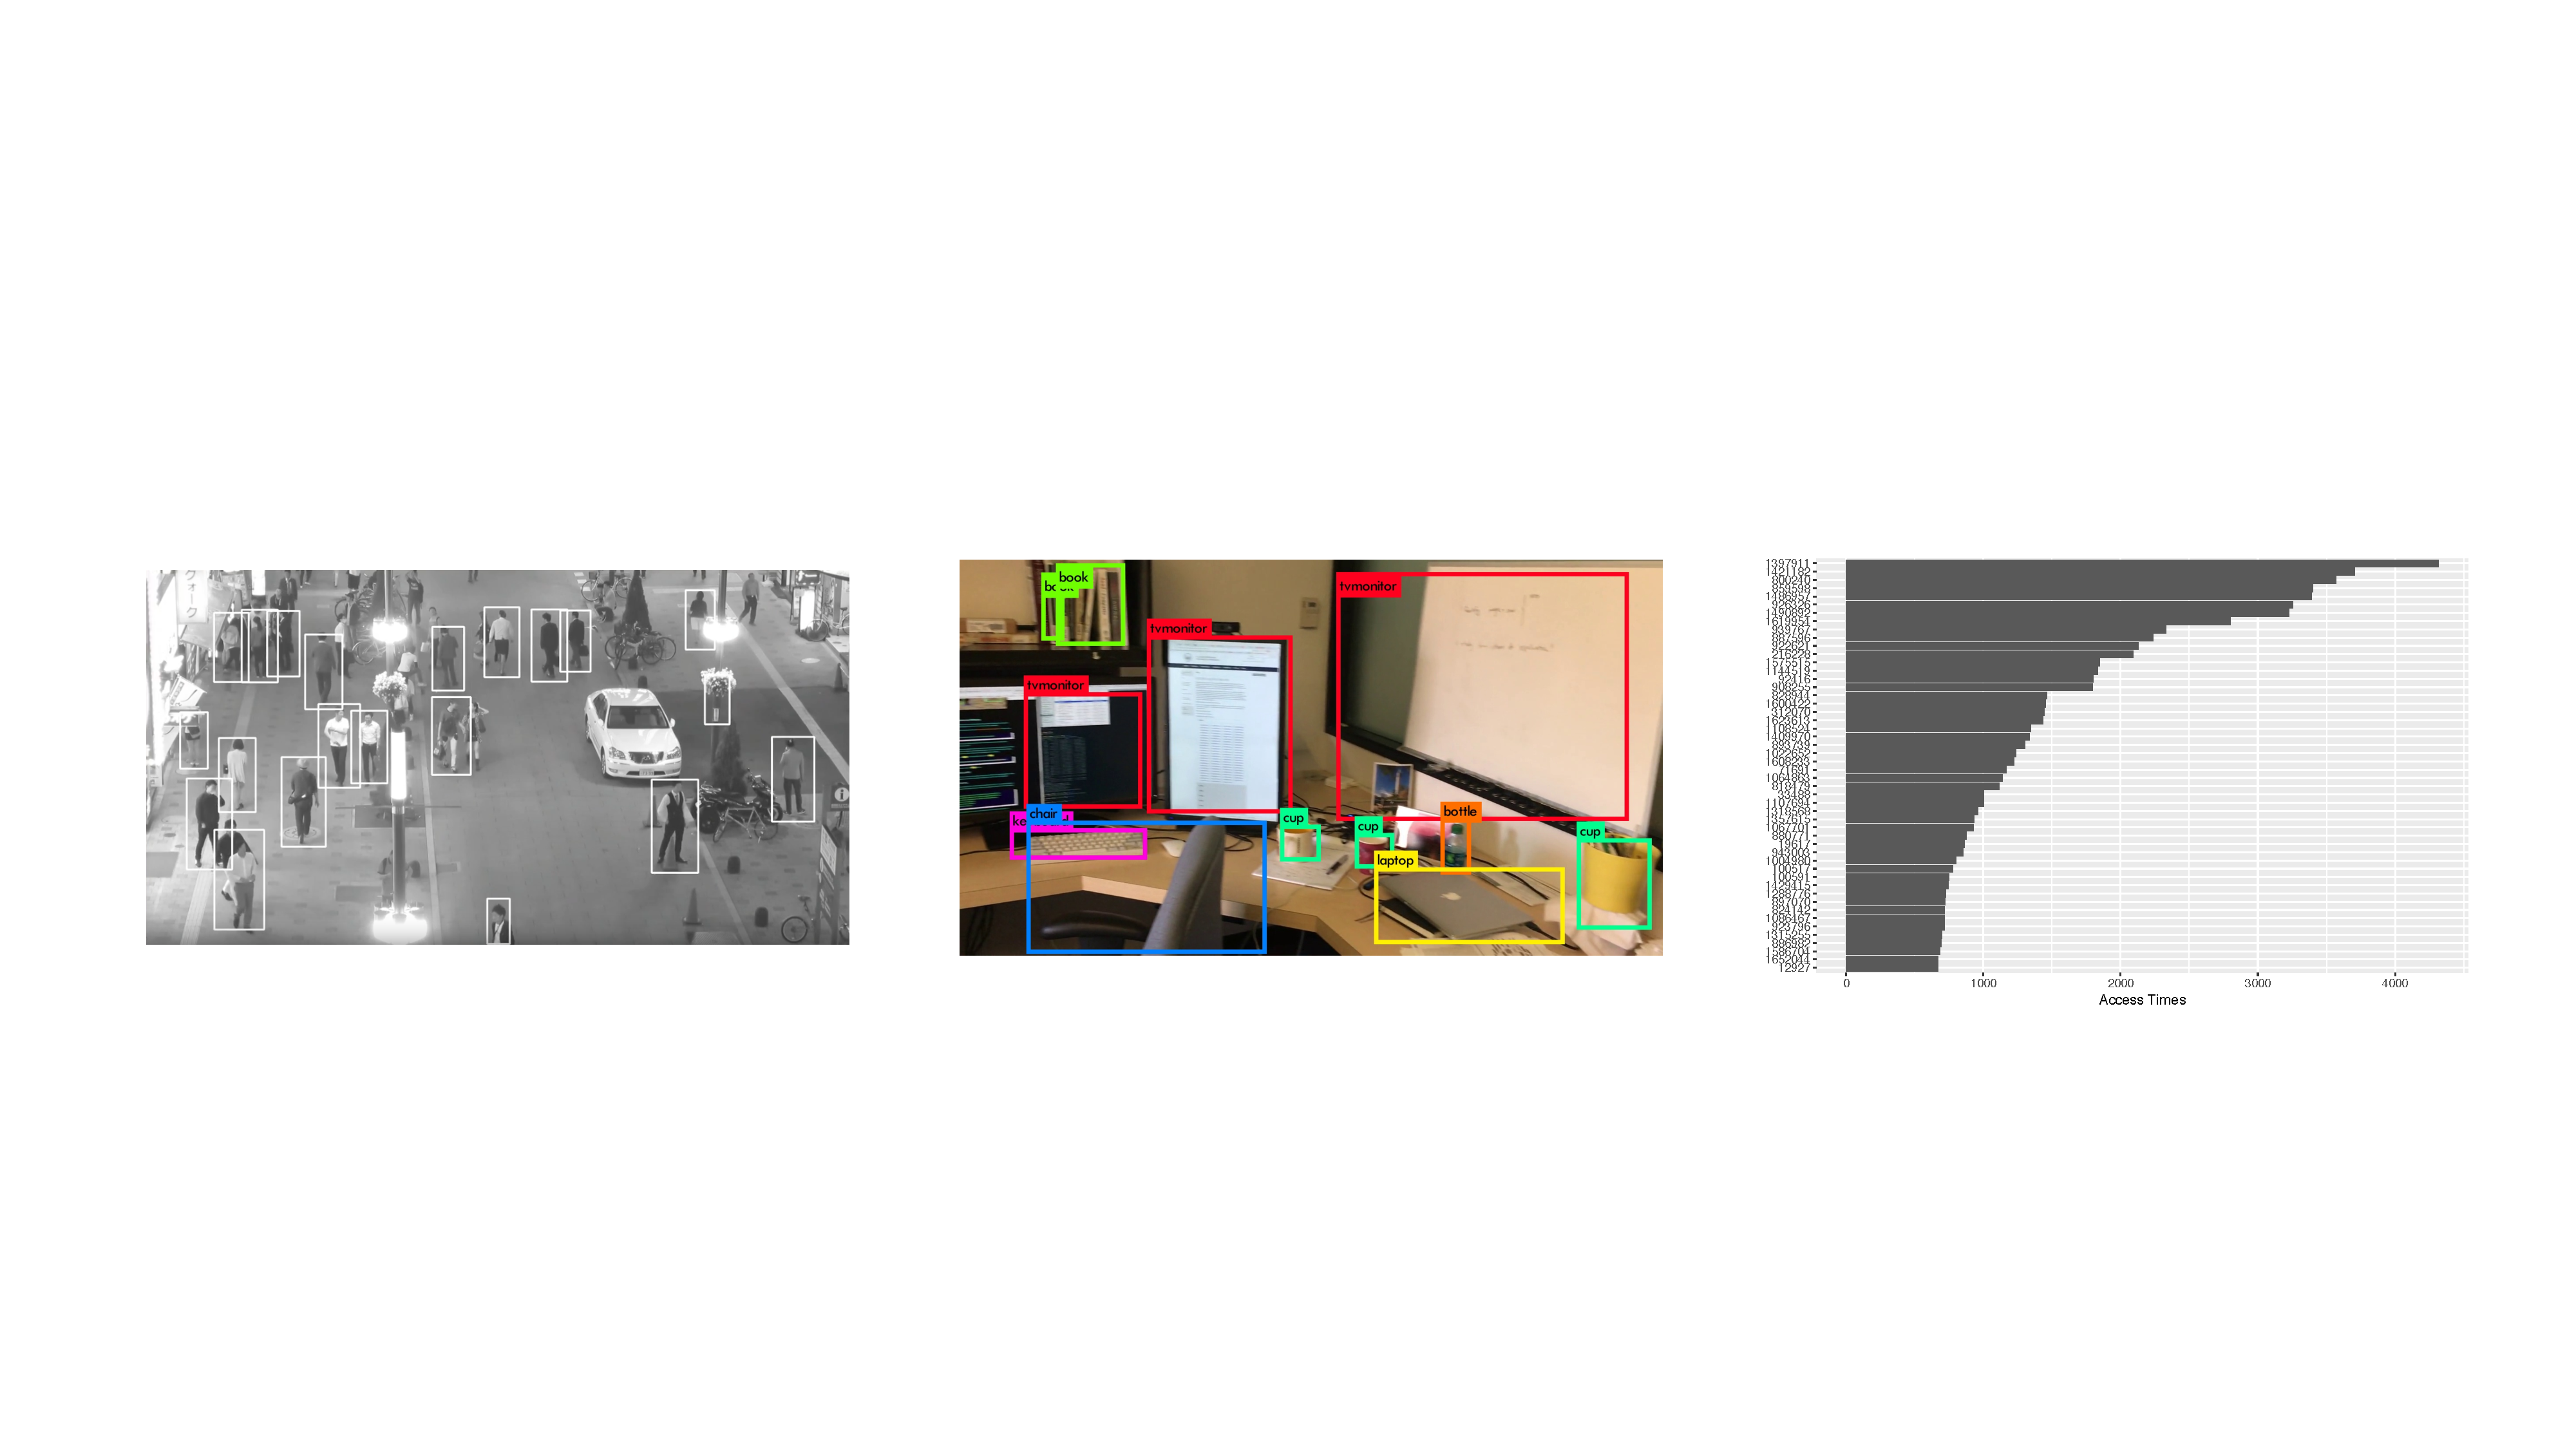
\includegraphics[width=\textwidth]{figures/apps.pdf}
  \caption{\sysname{} applications}
  \label{fig:apps}
\end{figure*}

Using \sysname{}, we've built three applications: pedestrian detection
surveillance, an augmented reality and a distributed Top-k.

\autoref{fig:apps} shows an illustration of these applications and the
application-specific part, including knobs, utility function and data set, is in
\autoref{tab:apps}. Below we describe each application in details.

\begin{table*}
  \small
  \centering
  \begin{tabular}{c c c c}
    \toprule
    Application & Knobs & Utility & Dataset \\
    \midrule
    Pedestrian Detection & resolution, framerate, quantizer
                        & F1 score & \begin{tabular}{@{}c@{}}MOT16-04 (training) \\
                                       MOT16-03 (testing)\end{tabular} \\
    \midrule
    Augmented Reality & resolution, framerate, quantizer & F1 score
                                  & \begin{tabular}{@{}c@{}} Video clips with
                                      iPhone \\
                                      office (training) \\
                                      home (testing)
                                    \end{tabular} \\
    \midrule
    Top-K & head (N), local threshold (T) & Kendall's W
                                  & \begin{tabular}{@{}@{}c@{}}
                                      \url{https://sec.gov} access log \\
                                      4 days (training) \\
                                      12 days (testing)
                                    \end{tabular} \\
    \bottomrule
  \end{tabular}
  \caption{\sysname{} Applications}
  \label{tab:apps}
\end{table*}

\para{Pedestrian detection:} This application analyzes video streams from
installed CCTV cameras and detect pedestrians inside. The detection result is a
list of bounding boxes (rectangles) representing pedestrian's relative location
within the view. Variant of this application can be used for safety monitoring,
anomaly detection or waiting line counting.

We implement most of the image-related operations with OpenCV
3.1~\cite{opencvlibrary}. Pedestrians are detected using histogram of oriented
gradients (HOG)~\cite{dalal2005histograms} with the default linear SVM
classifier. To ensure real-time processing of frames, GPU-accelerated
implementation is used in favor of the CPU-based implementation.

For video encoding, H.264 scheme is chosen for its prevalence in existing
systems. Our implementation is based on GStreamer~\cite{gstreamer}, using
\texttt{x264enc} plugin. To integrate with \sysname{}, we first create a
pipeline that exposes \texttt{appsrc} (to feed raw image data) and
\texttt{appsink} (to get encoded bytes). The GStreamer main loop is managed in a
separate thread and \sysname{} communicates with it via Rust's channel. The
\texttt{x264enc} is configured with \texttt{zerolatency} present and runs using
four threads. It uses constant quality encoding and the quantizer is exported as
a parameter that can be tuned: increasing the quantizer will degrade the image
quality.

Overall, this application has three degradation operations: reducing image
resolution, dropping frame rate or lower video encoding quality by adjusting the
quantizer.

For application accuracy measure, the detection results over degraded streams
are compared against a reference result where no degradation is in effect. A
successful detection is defined when the intersection over union (IOU), between
the detection and the reference results, is greater than
50\%~\cite{everingham2010pascal}. All the detection are combined and we use use
F1 score (\%) as the final accuracy. It represents the harmonic mean of
precision and recall, and has been used commonly in computer vision
tasks~\cite{Rijsbergen:1979:IR:539927}.

\para{Augmented Reality:} We target at mobile augmented reality applications
which offload the heavy computation to resources elsewhere. Although local
computation is gaining attraction~\cite{satyanarayanan2009case, zhang2015cloud},
wireless communication link is also susceptible to capacity variation; our
adaptation techniques can be applied to the wireless domain.

We use a similar setup (OpenCV + GStreamer) as the pedestrian detection
application except the actual function that analyzes the stream. To recognize
objects, a pre-trained neural network model~\cite{darknet13} is used. The model
has been trained with ImageNet~\cite{krizhevsky2012imagenet} and is able to
recognize everyday objects. Similar to our first application, we use the
GPU-accelerated implementation for real-time processing.

Although the utility function here is also F1 score, the criterion for a
successful detection is more strict: true-positive depends not only on the IOU
criteria, but also the type of objects must be matched.

\para{Distributed Top-K:} Many distributed system monitoring applications
require to answer the ``top-k'' question~\cite{babcock2003distributed}, such as
the top-k most popular URLs or the top-k most access files. Naive methods of
transmitting all the raw log entries to the aggregation point is not feasible as
popular servers typically have millions of requests per second. Local worker
nodes can first perform a window-based transformation that generates data
summary, such as key-value pairs of \texttt{<item, count>}. However, even after
this operation, the data size could still be too large given most real-world
access patterns follow a long-tail distribution. There is a large-but-irrelevant
tail that is unnecessary to send.

We consider two degradation operations that individual worker node can perform:
(1) a local Top-\texttt{N} operation that shortens the list first; (2) a local
threshold \texttt{T} that further filters small entries. Obviously, these two
operations are not orthogonal to each other. Their impact on data size reduction
and quality degradation depends on the distribution of the actual
data. \autoref{fig:topk} illustrates one concrete example of the entire pipeline
and the effect of two degradations.  The final results are evaluated using
Kendall's W. The Kendall's W is a distance measure of the concordance between
two ranked list. It outputs a statistic measure ranging from 0 to 1,
representing no agreement to complete agreement,
respectively~\cite{abdi2007kendall}.

\begin{figure}
  \centering
  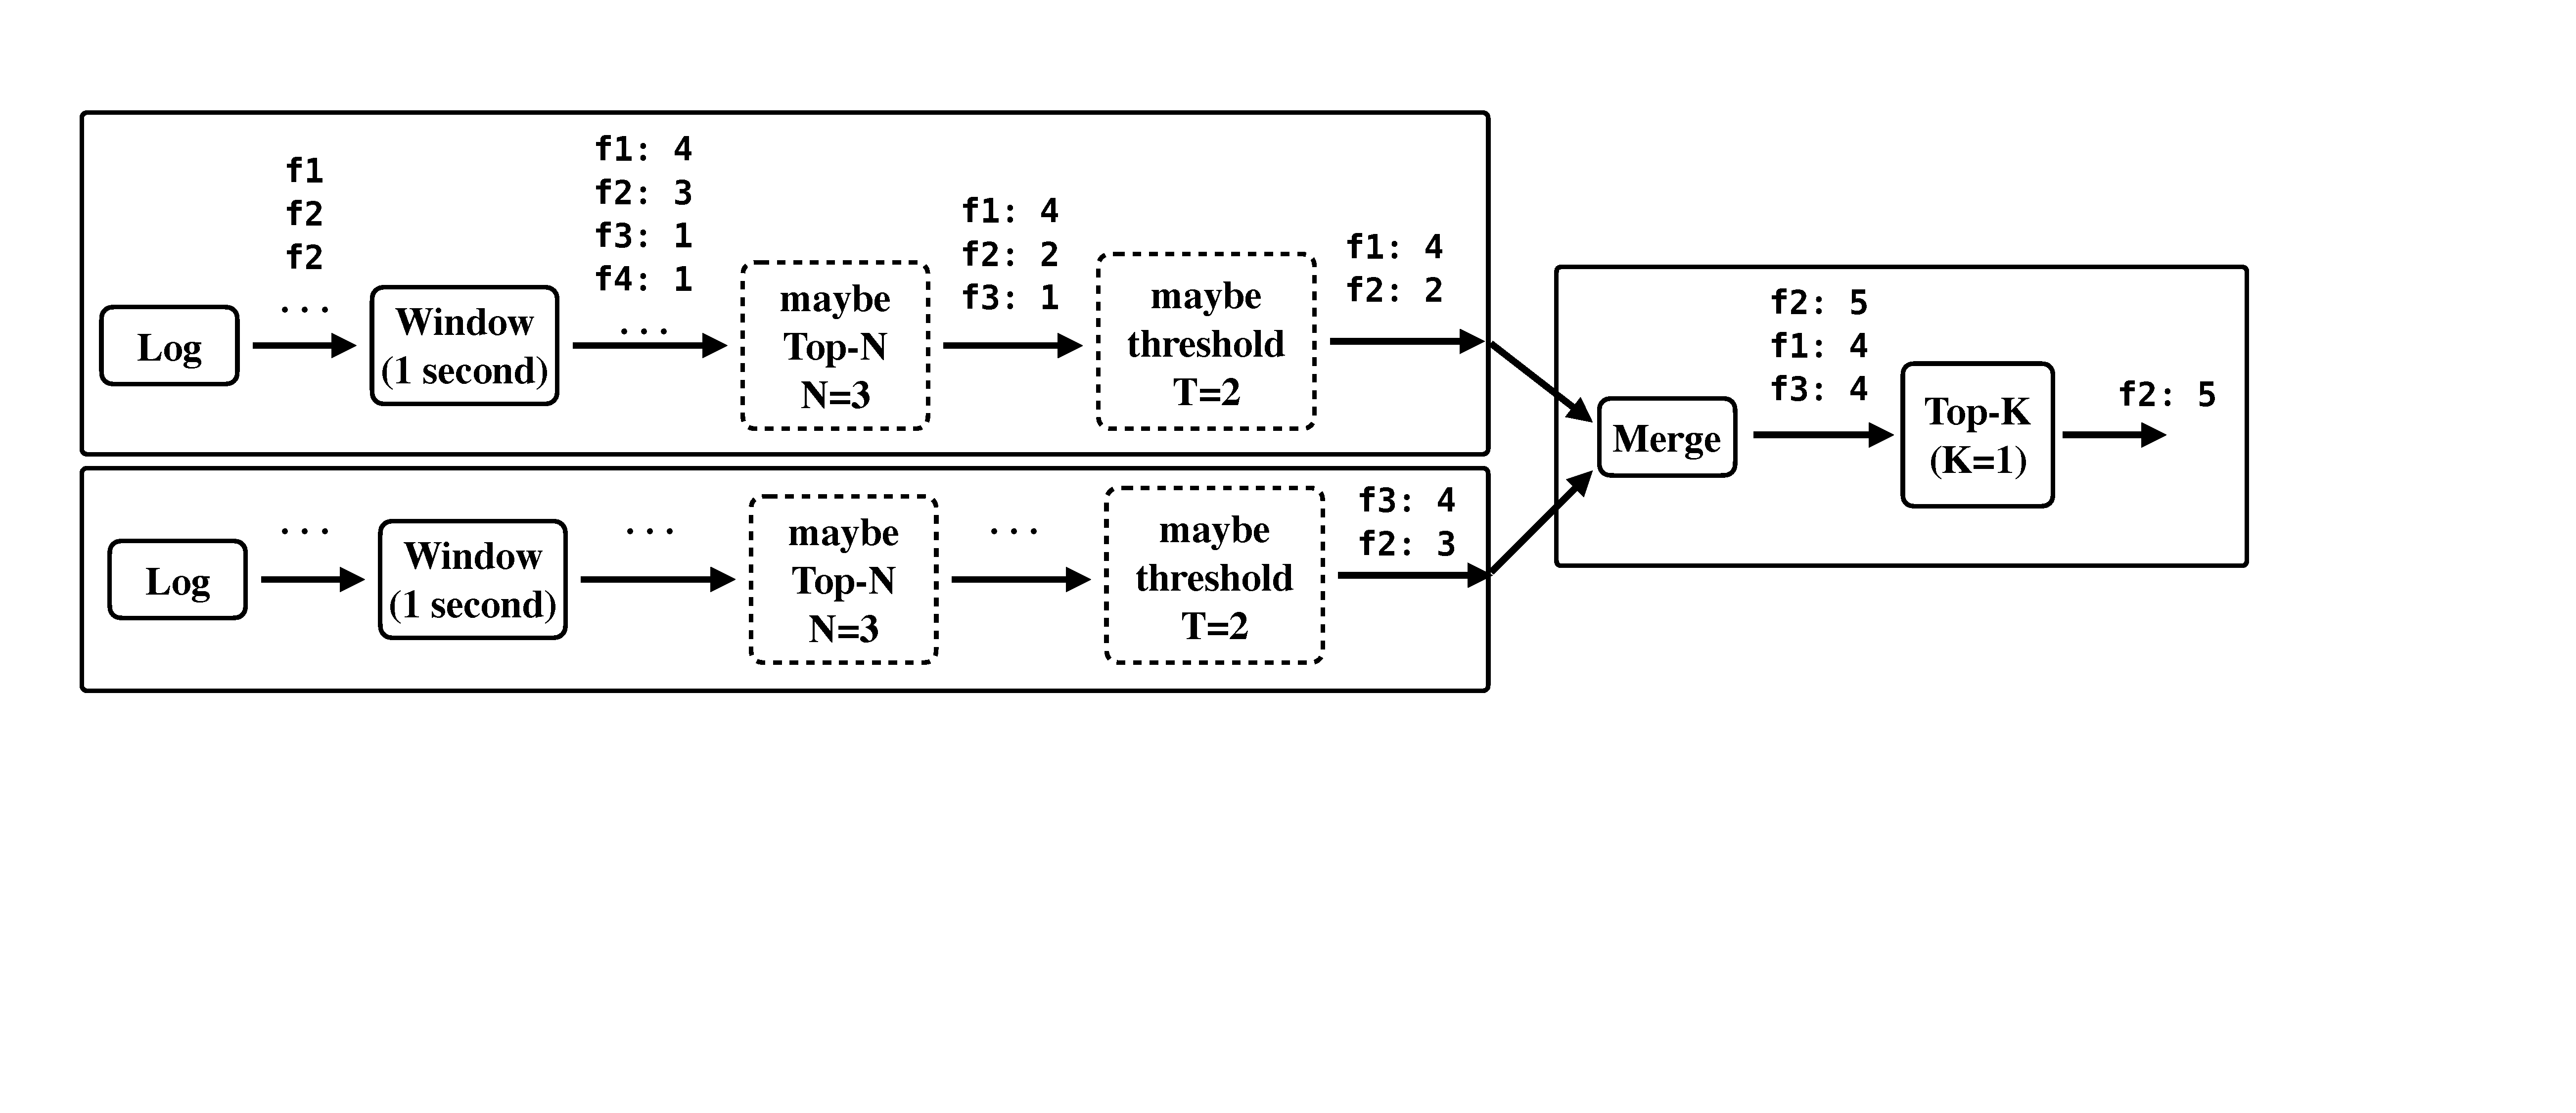
\includegraphics[width=\linewidth]{figures/topk.pdf}
  \caption{A distributed Top-K application has two tunable parameters: a local
    Top-N (N) and a local threshold (T).}
  \label{fig:topk}
\end{figure}

\section{Evaluation}
\label{sec:evaluation}

In this section, we first show the learned profile for each application. These
profiles serve as empirical evidence to back up the system design. Then for each
application, We show how they adapt the behavior at runtime. Under a controlled
experiment, even with only transient network capacity drop, our system is able
to maintain an end-to-end delay for 10 seconds in the wide-area and accuracy
level above 80\%. Application-agnostic protocols create significant backlogged
data (TCP for about 100 seconds) or unusable accuracy (UDP).

\subsection{Degradation Performance}
\label{sec:degr-perf}

\begin{figure}
  \centering
  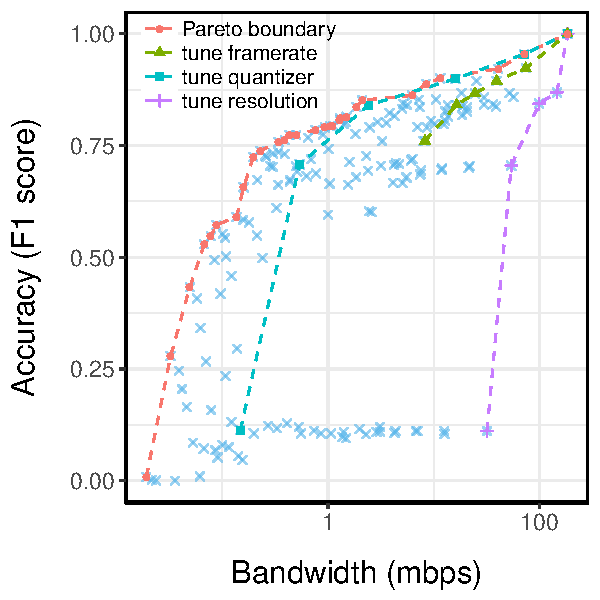
\includegraphics[width=0.6\textwidth]{figures/ped-profile.pdf}
  \caption{Bandwidth-accuracy tradeoff curve for pedestrian detection. Every
    point has a coordinate $(B(c), A(c))$ where $c$ represents one specific
    degradation configuration. The goal of the profiling is to obtain the Pareto
    boundary as an optimal degradation strategy. We also show the profile if
    only one degradation operation is involved, e.g.\,only tune the frame rate,
    only tune the quantization or only tune the resolution. These profiles with
    one dimension tunable have a sub-optimal performance in comparison to
    strategies that involve multiple dimensions.}
  \label{fig:pd-profile}
\end{figure}

\begin{figure}
  \centering
  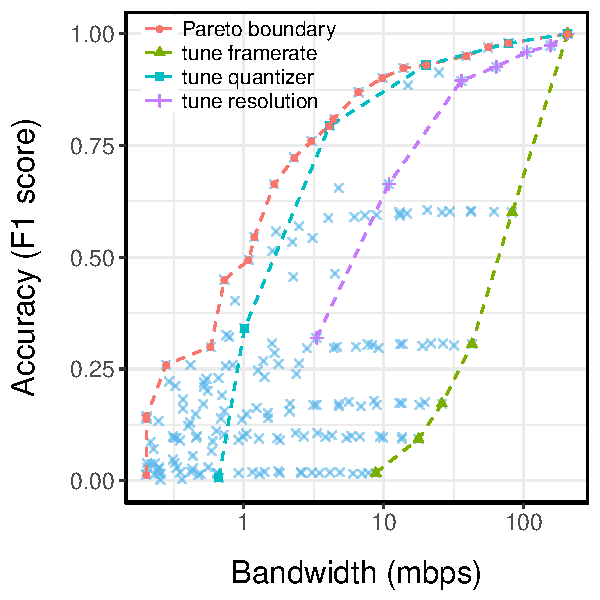
\includegraphics[width=0.6\textwidth]{figures/darknet-profile.pdf}
  \caption{Bandwidth-accuracy tradeoff curve for Augmented Reality. This figure
    has a similar setup as \autoref{fig:pd-profile} except the degradation
    profile has a different behavior.}
  \label{fig:ar-profile}
\end{figure}

\begin{figure}
  \centering
  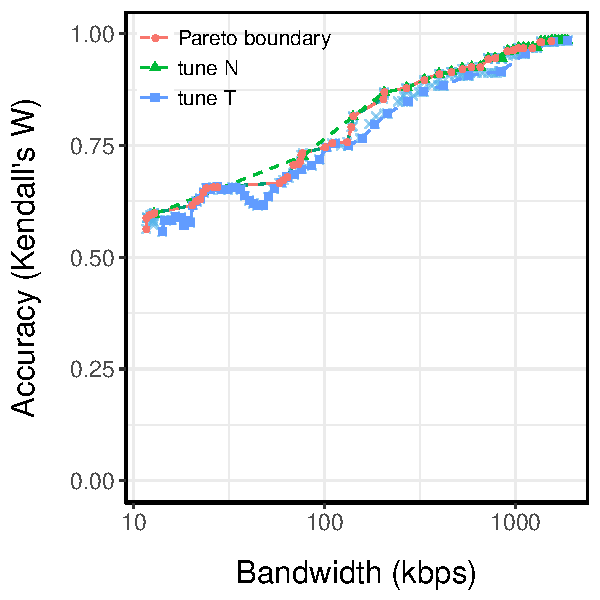
\includegraphics[width=0.6\textwidth]{figures/log-profile.pdf}
  \caption{Top-k}
  \label{fig:tk-profile}
\end{figure}

We describe the dataset we used for each application and then discuss what we've
learned from each result.

\para{Pedestrian Detection:} We use MOT16 dataset~\cite{milan2016mot16} to
evaluate this application. Specifically we used MOT16-04 as the training
dataset. The video feeds capture a busy pedestrian street at night with an
elevated viewpoint. The original resolution is 1920x1080, with frame rate
30. The training dataset has 1050 frames in total, amounting to 35-second
monitoring. On averge there are 45.3 people per frame.

There are three knobs in this application: resolution, frame rate and encoding
quality. To maintain the same 16:9 aspect ratio with the original 1920x1080
resolution, the resolution degradation only uses common 16:9 settings: 1600x900,
1280x720, 960x540 and 640x320. For the framerate, integer values are chosen in
favor of fraction values. The original frame rate is 30, and our degradation
explores 10, 5, 3, 2, 1. To adjust the video encoding quality of H.264, we vary
the encoding quantizer. The quantizer has a range from 0 (lossless) to 51 (worst
possible), and just for reference, 18 is the visually lossless
setting~\cite{bellard2012ffmpeg}. In our experiment, we use 10, 20, 30, 40, 50
as degradation parameters.

The generated profile is shown in~\autoref{fig:pd-profile} with x-axis being the
required bandwidth and the y-axis being the accuracy (F1 score). Each point in
the scatter plot represents one configuration that our offline profiling has
evaluated. Notice the vast spread in bandwidth requirement among configurations
with similar accuracy as well as the wide spread in accuracy among
configurations that consumes similar bandwidth.

We annotate three lines with configurations that only have one degradation
operation in effect. Notice the distinct behavior of these three lines: reducing
the resolution has the most penalty because the HOG detector has a minimal 128
pixels by 64 pixels window. The camera is deployed in a far-field context such
that scaling down the image will quickly affect the detection rate. Tuning frame
rate doesn't harm the accuracy too much. In fact, even with 1 FPS, the accuracy
is still relatively high (75\%). However, reducing frame rate alone doesn't
bring much bandwidth saving as the data size of each frame increases (as we have
mentioned in \autoref{fig:h264}). The most effective way that reduces the
bandwidth while preserving the accuracy is to adjust the quantizer because it
has an effect on every pixel. But adjusting the quantizer alone quickly leads to
accuracy drop because edge information is lost with an aggressive
quantization.

The Pareto boundary, or \textit{profile}, is the most important curve. Starting
from the right side, we see how the profile is close to the curve when only
quantizer is tuned; and for the case of more limited bandwidth, the most optimal
strategy is alone: it's only achievable with a combination of the three
operations.

\para{Augmented Reality:} For this application, we've collected training data
and test data by ourselves. The training data set is a 23-second video clip with
1920x1080 resolution and 30 FPS. It's taken on a mobile phone in an office
environment. The test data is 37-second in a home environment. During the
capture, we change the camera view in a slow pace to emulate how a real user
would look around the environment. Because target objects are relatively close
to the camera, we hypothesize that the profile for this application will has a
less accuracy drop if frame resolution is degraded; instead, due to the movement
of the camera, reducing frame rate will have a detrimental effect.

The generate profile is shown in \autoref{fig:ar-profile}. We do see a quick
degradation when the frame rate is tuned. The resolution degradation has a
modest effect and still, tuning the quantizer is mostly optimal up to a
point. The Pareto boundary is only achieved when multiple degradations are in
effect.

\para{Top-K:} To evalute the top-k application, we generate synthetic dataset
based on real-world access logs (EDGAR log file dataset, the access log of
\url{https://sec.gov} server). The original log file contains CSV-format data
extracted from their Apache web servers~\cite{edgarlog}. Because the original
log has only 500k access per hour, which is rather small in comparison to
today's CDN log, we condensed each hour-long data into one second as our
training and test data. After performing the local aggregation, the data size is
reduced from 500k entries per second to 50k key-value pairs (10x reduction).
Further reductions are made possible with the two degradation operations. The
parameter \texttt{N} ranges from 100 to 15000 while \texttt{T} is from 0 to 500.

\autoref{fig:tk-profile} shows the generated profile. As we can see, most
configurations are very close to the Pareto boundary. The Pareto boundary is
mostly achieved by tuning \texttt{N}. If applied for a different data set, this
result may be different.

\subsection{Runtime Performance}
\label{sec:runtime-performance}

\begin{figure}
  \centering
  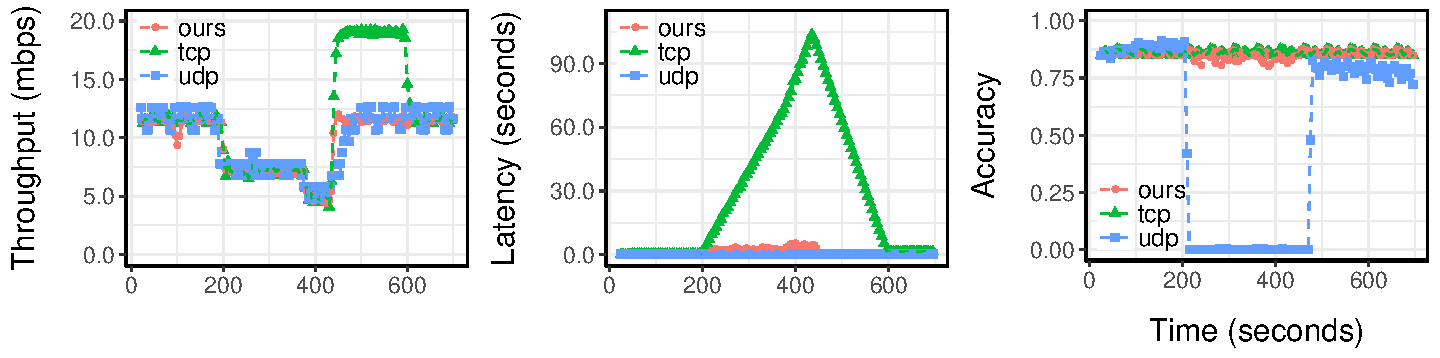
\includegraphics[width=\textwidth]{figures/ped-runtime-horizontal.pdf}
  \caption{Runtime adaptation for pedestrian detection. The leftmost figure
    shows the throughput according to the receiver before and after we apply
    traffic shaping; note how TCP is catching up at 440s when the traffic
    shaping is removed. The middle figure shows the latency using three
    strategies, especially the increased latency for TCP when network capacity
    drops. The rightmost figure shows the accuracy. During the traffic shaping,
    UDP is experiencing a severe packet loss that many frames failed to be
    recovered.}
  \label{fig:ped-runtime}
\end{figure}

To evaluate the runtime behavior of \sysname{}, we conduct controlled
experiments using four geo-distributed worker nodes from Amazon EC2
(\textit{t2.large} instances) and an aggregation server from our institute. For
each experiment, worker nodes transmit test data for about 10 mins. During each
session, we use Linux \texttt{tc} utility to adjust outgoing bandwidth to
experiment with network resource variation.

We compare our system with baseline systems that directly uses TCP and UDP. In
all three applications, the raw data streams are orders of magnitude
larger. While our system can adapt the rate, it could be unfair to baseline
solutions. We've adjusted the default degradation operation so that TCP and UDP
would work just fine under the normal conditions; in this way, we make a fair
comparison and study how the adaptation behaves. In the case of UDP, shaping at
the source doesn't emulate the packet loss behavior with out-of-order
delivery. We use \texttt{netem} to control packet loss rate to match the desired
shaping characteristics in the wide-area.

The results are shown in \autoref{fig:ped-runtime} and
\autoref{fig:cdn-runtime}.\footnote{The augmented reality application exhibits a
  similar behavior as the pedestrian detection. However, due to time constrain,
  the entire experiment is not finished.}  In our experiments, we see long
delays in TCP when the network bandwidth is limited. The latency increases
linearly after the traffic shaping starts. When the bandwidth shaping stops, TCP
quickly fills the connection to recover. Depending on the queued size, the
recovery could take a few minutes or tens of seconds. For UDP, the latency has
been consistently small (mostly below 1 second) because there is no queue
building up. But when traffic shaping starts and packet loss occurs, the
accuracy drop is catastrophic.

Applications built with \sysname{} perform with a middle-ground behavior between
the two extremes: a bounded latency with a reasonable accuracy drop. We notice
that the top-k application still has about ten seconds delay. The reason for the
slow adaptation in this application is two-folds: (1) our current implementation
only requests for bandwidth information when congestion is detected, the delay
of getting bandwidth estimation can be large in the case of network capacity
drop; (2) we perform the bandwidth estimation in a conservative way with
exponential smoothing to avoid sudden changes. While more improvements are
possible (and we plan to achieve it), the current results have demonstrated the
effectiveness of trading data fidelity for data freshness well.

\begin{figure}
  \centering
  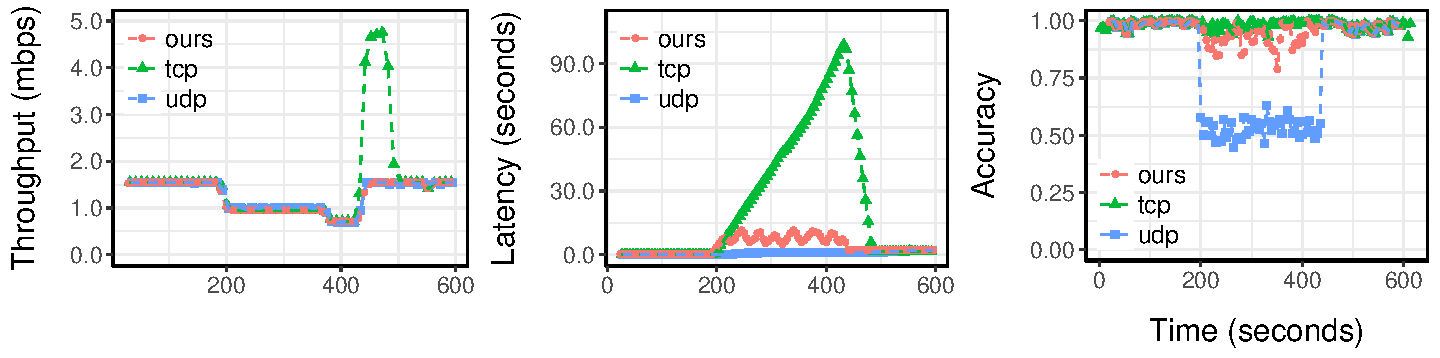
\includegraphics[width=\textwidth]{figures/cdn-runtime-horizontal.pdf}
  \caption{Runtime Adaptation of Top-K}
  \label{fig:cdn-runtime}
\end{figure}

%%% Local Variables:
%%% mode: latex
%%% TeX-master: "thesis"
%%% End:
